\subsection{Middleware}


\paragraph{Notation}
When talking about middleware and Elixir, we will often use the term
\textbf{process} instead of lightweight thread, as well as \textbf{application}
in place of ``architectural macro-component''.
We will strive to adhere
to the Erlang/Elixir notation, which has these old fashioned/slightly inaccurate
names since it was born and developed for another context, i.e., telephony.


\subsubsection{Applications}

This section presents the middleware services.

An overview to the organization of the middleware components is given in Figure
\ref{fig:mw-arch-over}. The picture is both a dependency and an information flow
graph: if a service $A$ is above another one and has a downward connection
which touches service $B$, then $A$ both depends and sends messages to $B$.
We designed this structure in order to avoid circular dependencies among
services and to be able to reason clearly about an actor-model based system.
\\

Also, it is possible to send a message to a module which may seem
unreachable: the sender can hand the message off to the
forwarder, asking to delivery it to a loopback queue.
This mechanism has to be used carefully to avoid infinite loops. Therefore
we restrict its usage to specific situations.

\begin{figure}[H]
  \centering
  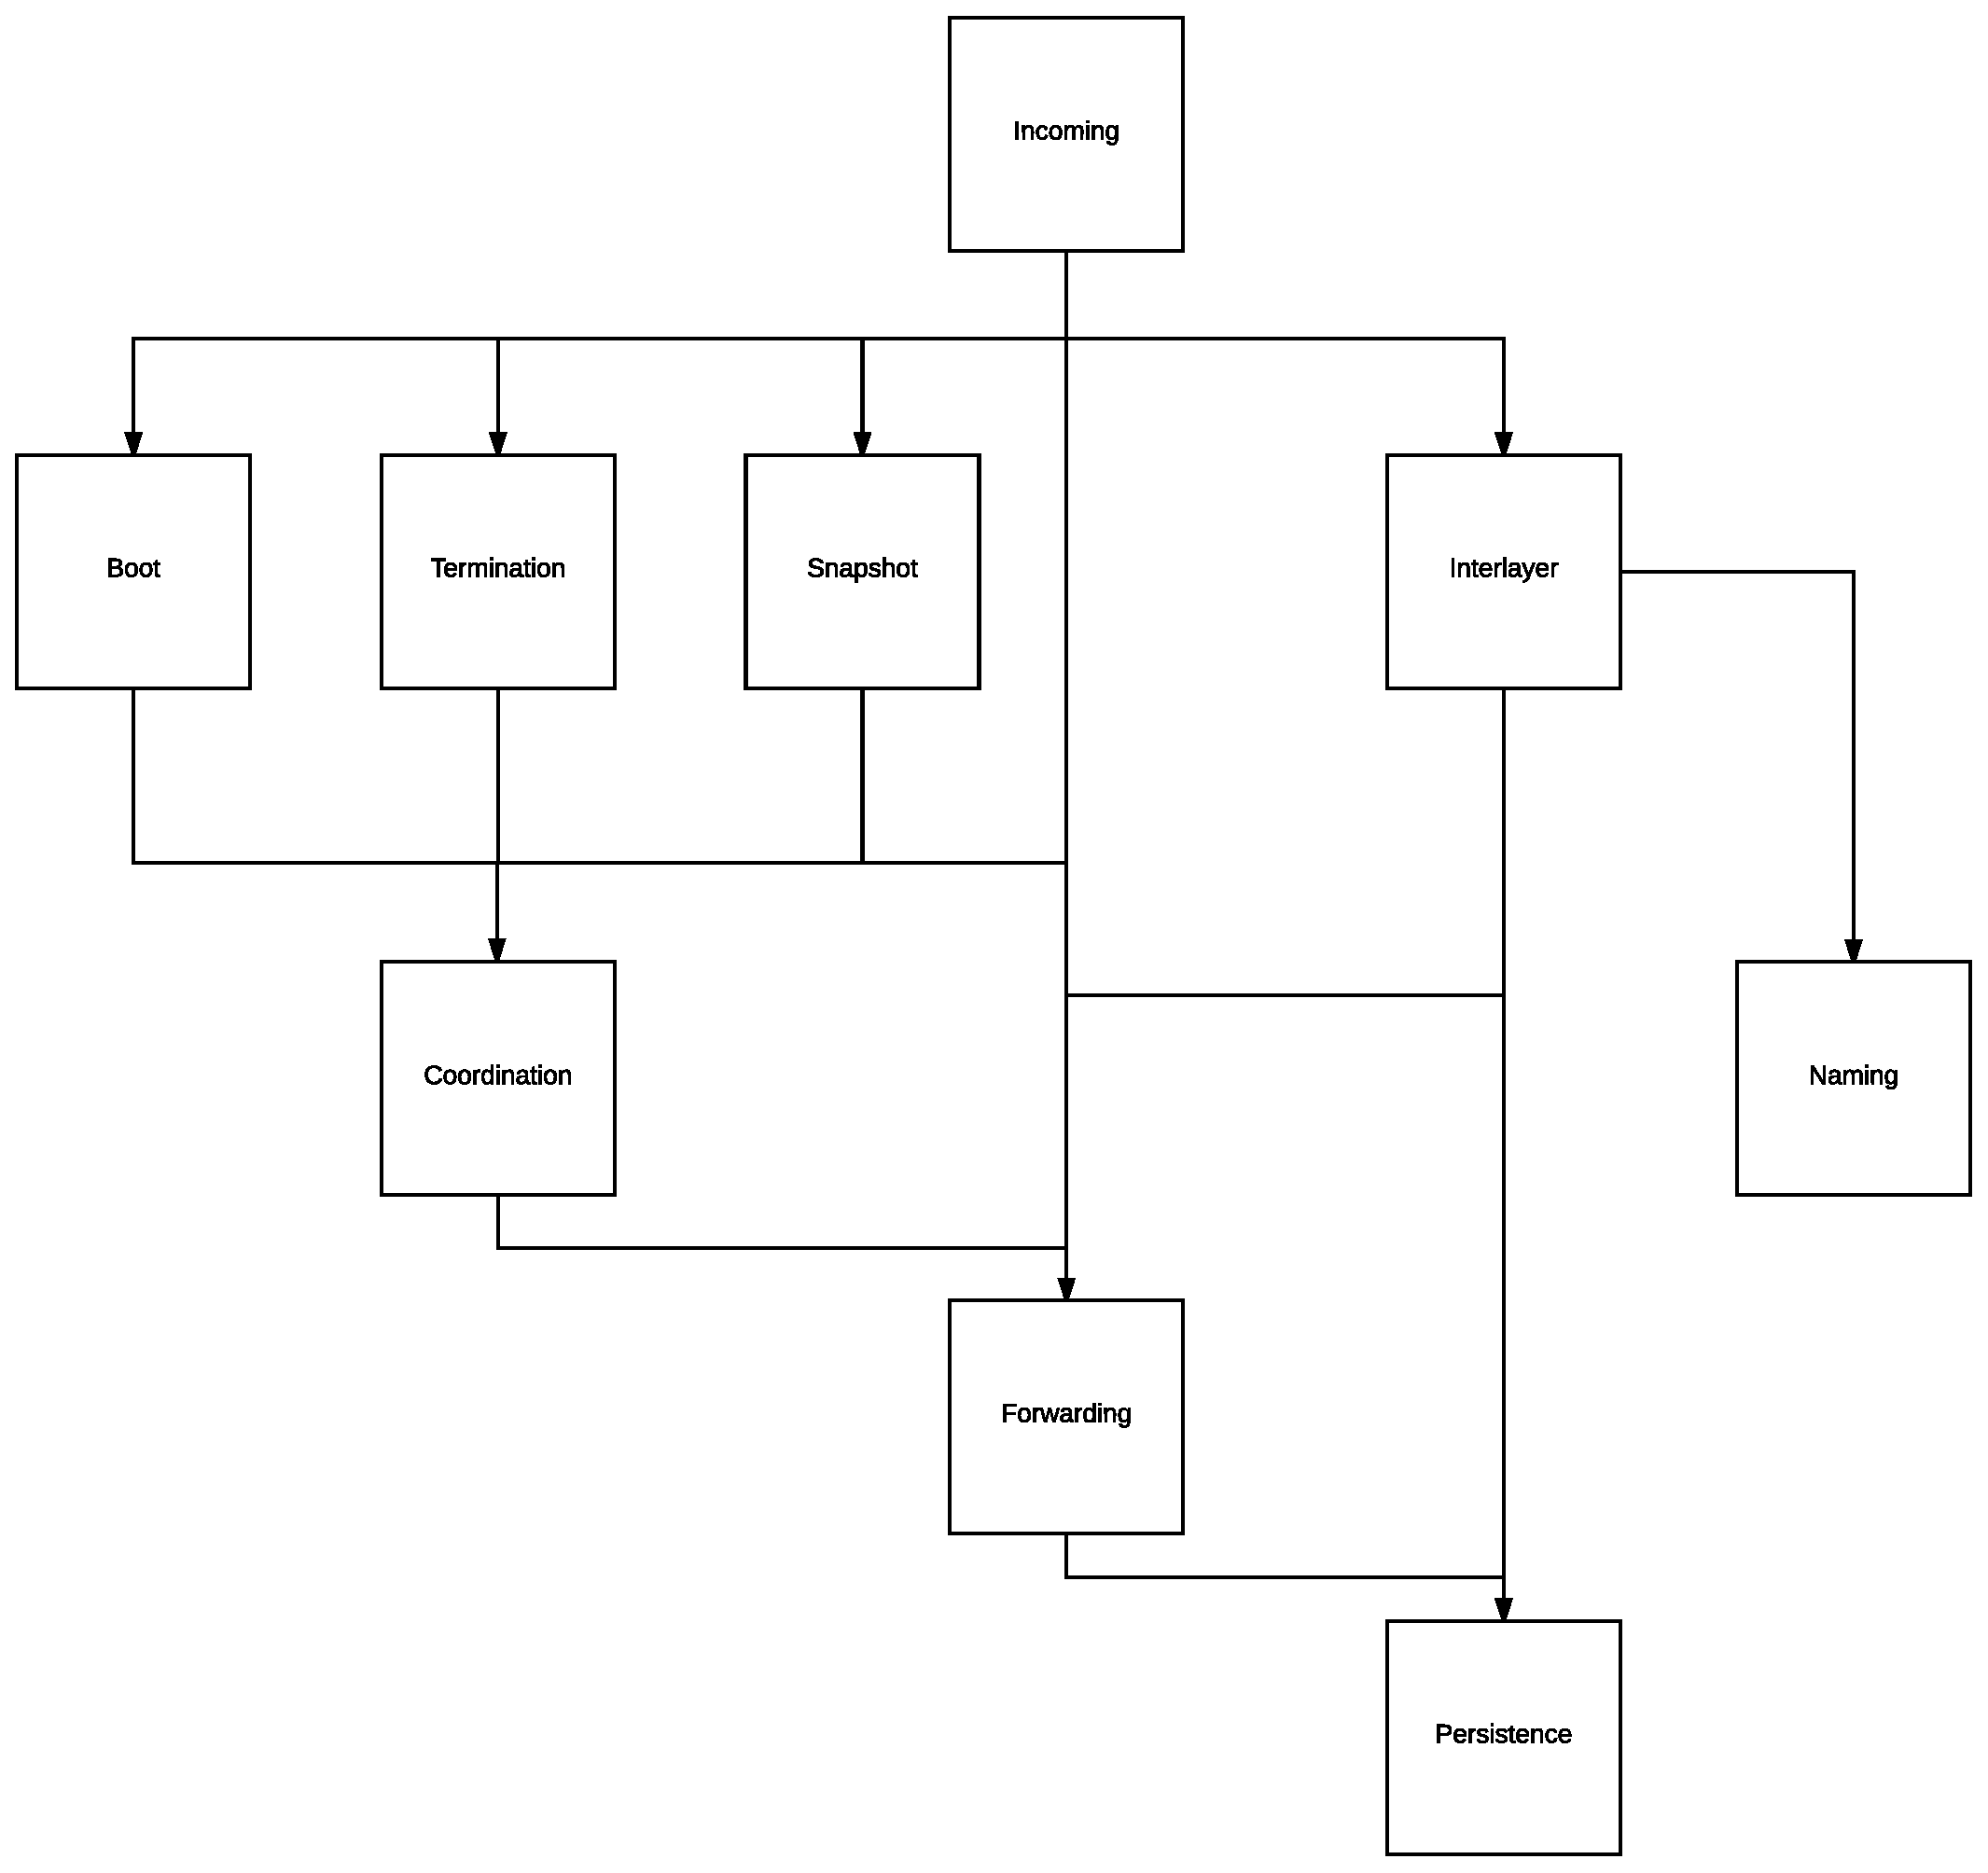
\includegraphics[height=9cm]{images/solution/mw/overview.eps}
  \caption{Middleware architecture overview}
  \label{fig:mw-arch-over}
\end{figure}

% \begin{itemize}
%   \item \texttt{naming}: service that provides a correspondence between logic
%     names and their actual location;
%   \item \texttt{forwarding}: service that represents the abstraction through
%     which it is possible to deliver messages to other middleware nodes;
%   \item \texttt{incoming}: service that is responsible of handling messages
%     coming from other middleware nodes;
%   \item \texttt{interlayer}: service that represents the interface between
%     the application and middleware layers;
%   \item \texttt{boot}: service that is responsible to start the system neatly;
%   \item \texttt{termination}: service that shut downs the node and the system
%     gracefully;
%   \item \texttt{snapshot}: service that takes consistent views of the node and
%     the system;
%   \item \texttt{coordination}: service that coordinates the interaction among
%     the nodes of the system;
%   \item \texttt{persistence}: service that provides a set of utilities to
%     store data in a persistent way.
% \end{itemize}

\subsubsubsection{Naming service}
The Naming service, fed with an reactive
entity id and its type, finds the node on
which a given reactive entity resides.

This is completely decoupled from the application
layer, which just provides the identifier and the type of the entity in the
headers of the message handed over to the middleware. Then, the
Naming component just have to look up for the node on which the reactive
entity resides through a local configuration file.

\subsubsubsection{Forwarding service}
The Forwarding service delivers messages to other nodes. This component
comprise just an interface (\texttt{MQProxy}) and its
implementation (\texttt{RabbitSender}).

Basically, a \texttt{RabbitSender} takes a message as input and guarantees to
send it to the intended recipient, which could be middleware node or a
RabbitMQ pub/sub queue shared with the other message brokers.
\texttt{RabbitSender}s are able to make this decision by simply looking if the
messages they are handling are events or communications between districts.
In the former case, the messages are propagated towards the frontend of the
application (and therefore to the brokers). In the latter case, the messages are
sent to the district specified as the recipient of the message.

\subsubsubsection{Incoming service}
The Incoming service is responsible of receiving messages from other
middleware nodes and to dispatch these messages to the appropriate middleware
service.
However, before dispatching this component process the message by applying some
checks: in fact, a message may be directed to another node or it might have to
be withheld if a snapshot is occurring.

Therefore, we decided to take advantage of Elixir's
\href{https://hexdocs.pm/gen_stage/GenStage.html}{GenStage} behaviour and
structure the modules of this component as a pipeline through which the
message is processed:

\begin{figure}[H]
  \centering
  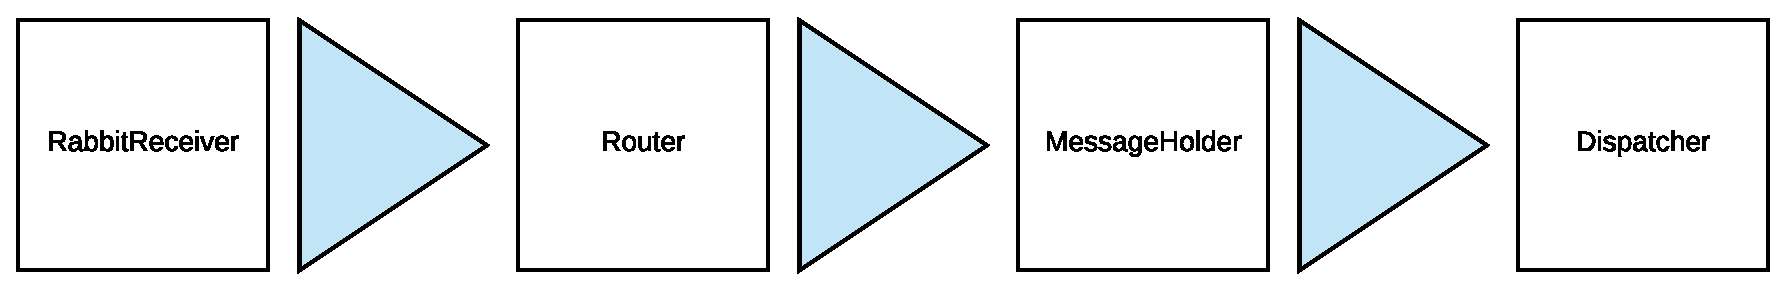
\includegraphics[width=\columnwidth]{images/solution/mw/inc/architect.eps}
  \caption{Incoming pipeline}
  \label{fig:mw-incoming}
\end{figure}

\begin{itemize}
  \item A RabbitReceiver is a process which receives messages from a single
    adjacent middleware node (or ``neighbor'') using RabbitMQ
  \item A Router compares the recipient field of the message with the
    identifier of the current node. If it is different, then it forwards the
    message to the next node along the path to the recipient
  \item A MessageHolder prevents messages to reach the dispatching point if a
    snapshot is happening. Then, when the snapshot ends, the messages will be
    forwarded again towards the Dispatcher
  \item A Dispatcher dispatches messages to a given service of the middleware
\end{itemize}

\begin{figure}[H]
  \centering
  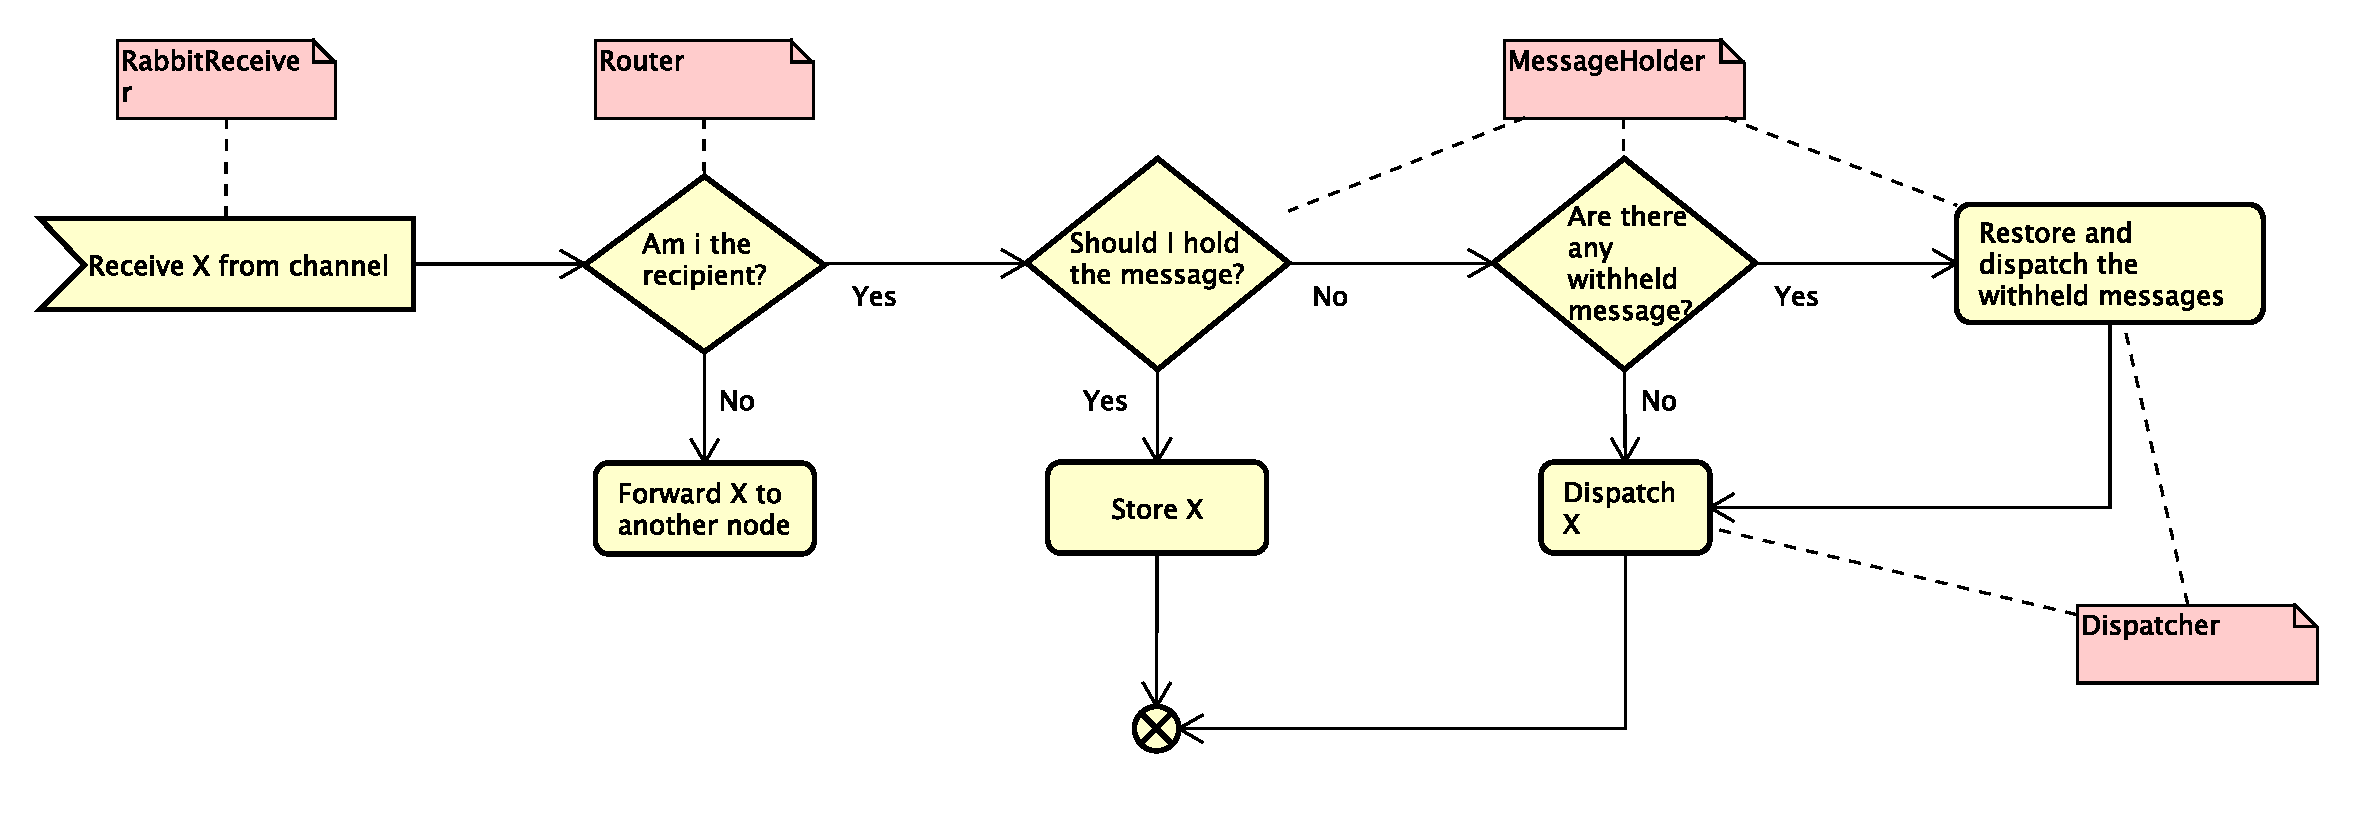
\includegraphics[width=\columnwidth]{images/solution/mw/inc/activity.eps}
  \caption{Activity diagram for Incoming pipeline}
  \label{fig:mw-incoming-activity}
\end{figure}

Thanks to the flexibility of GenStage, we can compose our pipelines by adding
an arbitrary number of elements at each stage of the pipeline. For instance,
there is one RabbitReceiver for each middleware neighbor plus one for loopback
communication: in this case, we just have to spawn as many RabbitReceivers as
needed and then make the Router subscribe to the events generated by them
(that is, the incoming messages).

\subsubsubsection{Interlayer service}

This component is responsible of the communication that is performed between
different layers, namely the one which it belongs (the \textbf{middleware}) and
another one who uses the middleware layer, that is the \textbf{application}
layer.

We show in Figure \ref{fig:mw-interlayer} the architecture of this service and
then we will show in detail each module that composes this component.

\begin{figure}[H]
  \centering
  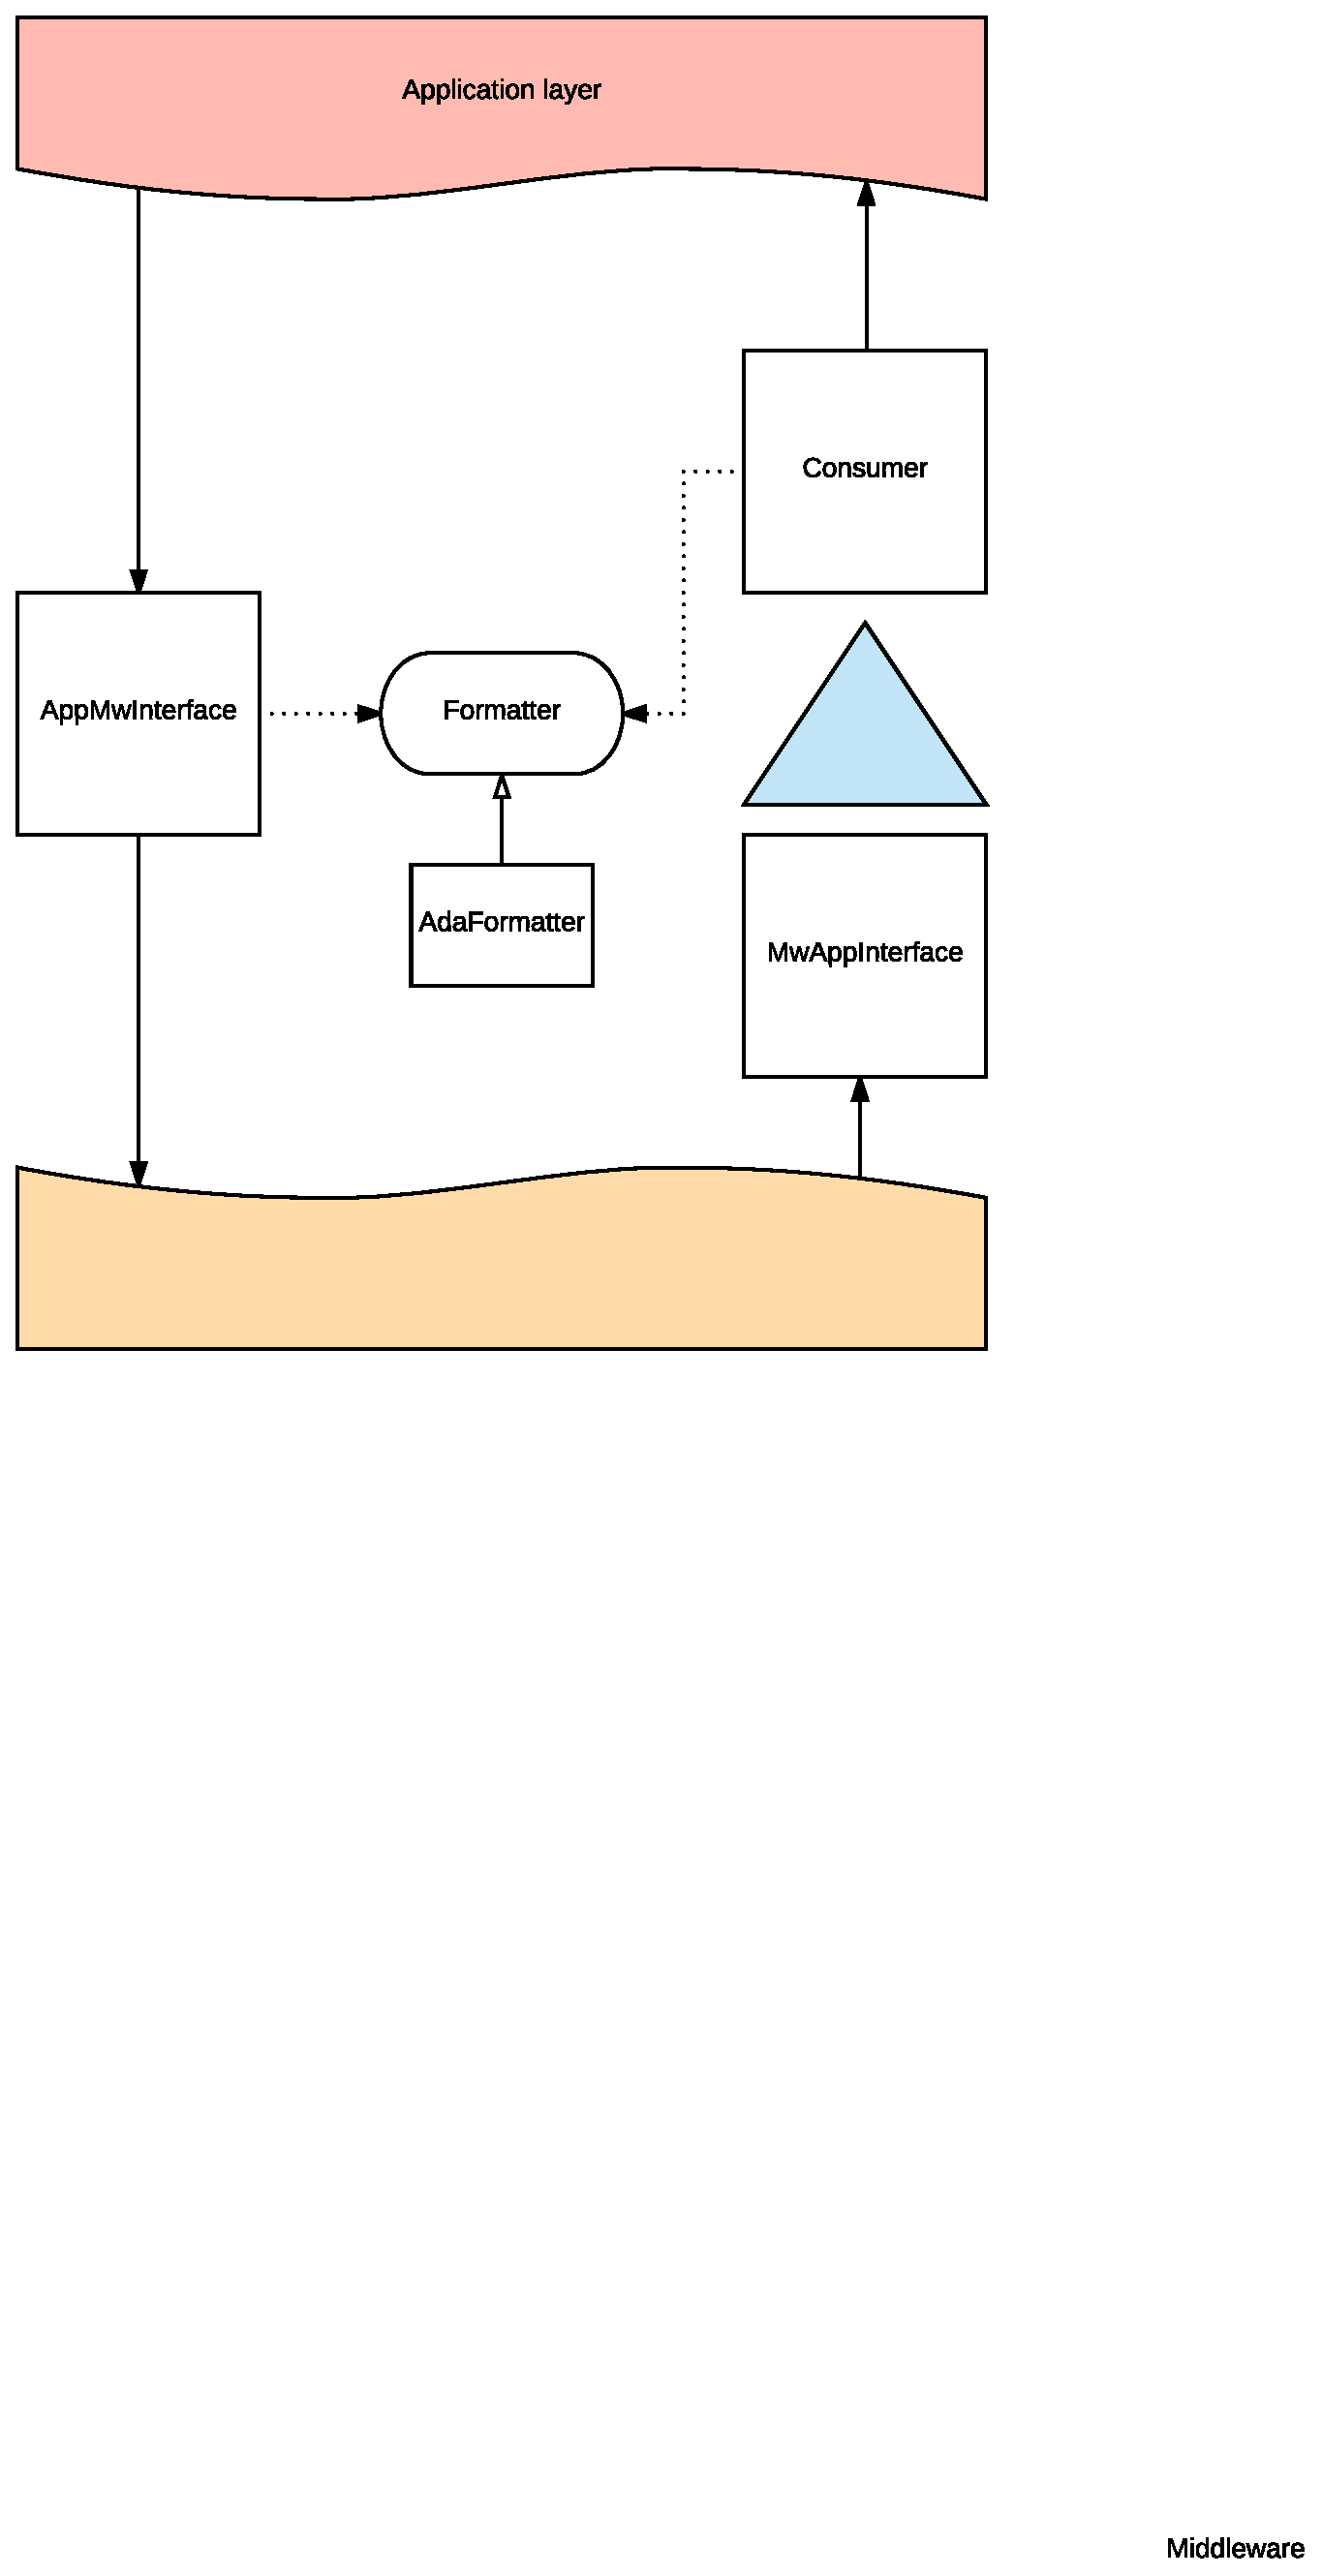
\includegraphics[width=.8\columnwidth]{images/solution/mw/int/architect.eps}
  \caption{Middleware's Interlayer service}
  \label{fig:mw-interlayer}
\end{figure}

We can see that the Interlayer service embodies two flows of information, each
one directed in the opposite direction as the other (the orange band represents
the middleware).

The \texttt{AppMwInterface} module just listens on a port waiting for messages
from the application layer and passes them to other services in the middleware.
It is capable of receiving different messages in parallel.

\texttt{MwAppInterface} receives requests by other middleware services to send
messages to the application layer. Instead of blocking the requesting process
on the delivery of the message, the latter gets stored in a Redis queue and
asynchronously handed over to the \texttt{Consumer} module by means of the
GenStage behaviour. When they demand work, \texttt{Consumer} instances send
pending messages to the application layer and, for each successful delivery,
pop the delivered message from the Redis queue.

Also, \texttt{Consumer}s can store meta-information for messages delivered to
the application. They do so in order to keep track of the RPCs performed by the
application layer, namely storing the logical name of the node which issued a
request in a Redis map. Then, when an RPC gets satisfied from the
application layer, \texttt{AppMwInterface} will correlate the answer with the
node which initially issued the request, and will forward the RPC result to it.
In fact, this feature allows us to preserve the transparency offered by the
middleware in the case of application-level RPCs.

Since some runtimes may handle strings in a different format with respect to
what Elixir does, we defined a \texttt{Formatter} behaviour for cope with these
issues.
We implemented a couple of formatters, one for Elixir (it does nothing but
return the message as it is) and one for Ada. In particular, Ada does not
output the actual character sequence when using \texttt{'Output}: in this case
the receiving sockets reads additional meta-information along with the string,
which are basically the boundaries of the binary data streamed.
However, this is not enough: in fact, we also had to split long messages since
Ada's Stream \texttt{'Input} attribute reads up to about 200B; therefore, the
\texttt{Consumer} module also has to split long messages into chunks in order
to deliver them without causing a failure during the reception.

\subsubsubsection{Boot service}\label{sec:mw-boot-descr}

The Boot service is responsible of starting the system in a graceful fashion.
It does so by dividing the start phase into two subphases, namely the
\textbf{marker diffusion} and the \textbf{(own) boot} phase. The procedure is
the same shown in Figure \ref{fig:sys-bootstrap-protocol}, with the first phase
going from left to right and the second phase going in the opposite direction.

In this context, by \textit{marker} we will mean \textit{boot marker}.

When receiving a marker, this the Boot service will forward the marker to all
of its adjacent middleware nodes.
Then, when receiving further markers, this service will just reply immediately
with an end marker.

After having received all the replies for the markers, the Boot service will
request to the application layer to gracefully start.
When the application layer will inform the middleware it started, this service
will send an end marker to all of its adjacent middleware nodes.

\subsubsubsection{Termination service}\label{sec:mw-termination-descr}

The Termination service is responsible of shutting down the system in a
graceful fashion.
It does so by dividing the termination phase into two subphases, namely the
\textbf{marker diffusion} and the \textbf{(own) termination} phase. The
procedure is the same shown in Figure \ref{fig:sys-termination-protocol}, with
the first phase going from left to right and the second phase going in the
opposite direction.

In this context, by \textit{marker} we will mean \textit{termination marker}.

When receiving a marker, this the Termination service will forward the marker
to all of its adjacent middleware nodes.
Then, when receiving further markers, this service will just reply immediately
with an end marker.

After having received all the replies for the markers, the Termination service
will request to the application layer to gracefully shut down.
When the application layer will inform the middleware it has terminated, this
service will send an end marker to all of its adjacent middleware nodes.

\subsubsubsection{Snapshot service}
This component is responsible of taking global and consistent snapshots by
implementing the Chandy-Lamport algorithm with the help of the
\texttt{MessageHolder} module in the Incoming service, which holds the message
during the execution of a snapshot.

This service is comprehensive of three architectural units:

\begin{enumerate}
  \item \texttt{ChandyLamportSnapshot}, which is a wrapper for an on-going
        snapshot;
  \item \texttt{ChandyLamportExecutor}, which embodies the logic necessary to
        exchange (i.e., process and send) messages relative to the
        Chandy-Lamport procedure and keeps track of the current snapshots being
        taken;
  \item \texttt{ChandyLamport}: supervisor which instantiates, monitors and
        stops \texttt{ChandyLamportSnapshot} children on demand for the
        \texttt{ChandyLamportExecutor}
\end{enumerate}

\subsubsubsection{Coordination service}

This component is responsible of the supervising the life-cycle of an
application run on our middleware, so our backend is able to operate
cohesively.

There are just two architectural units which compose this service:

\begin{enumerate}
\item a \texttt{Coordinator} initiates the boot process when requested and the
  termination process when the time limit for the application elapses;
\item \texttt{Monitor}s supervise the status of some services. In
  particular, we instantiated two monitor processes, one for the boot process
  and another one for the termination process. If a process $X$ does not end
  within a pre-configured time limit (we arbitrarily set 15 seconds for this
  parameter) after being started, the monitor issues again a request to
  perform $X$.
\end{enumerate}

\subsubsubsection{Persistence service}

This component is an adapter towards persistence and caching services.

More specifically, persistence is a collection of Redix wrappers. Redix is an
Elixir client for Redis, which handles all the network communication and
provides simple and convenient API to access Redis services.
Therefore, we just have to specify some of the CRUD operations for a certain
data structure we are interested in -- it could be a map (e.g., for pending
requests, so that we are able to correlate an id to a given request) or a
queue (e.g., pending unsent messages directed to the application layer).

However, we stress the fact that even if Persistence service uses Redis, it
could have used anything else without changing its API (the persistence
technology we employed is completely transparent to the other middleware
services).



\subsubsection{Protocols}

\subsubsubsection{Application - Middleware}
This subsubsection describes the communication protocol between
the application (i.e., IL) and the middleware layer
\paragraph{Fire and forget}
It is a one-way message pattern (the service sends a message without expecting
a response). Since the application and the middleware will reside on the same
physical node, we can assume that the communication is reliable: once a message
is sent from the application layer it arrives to the middleware layer and
viceversa. The asynchronous communication decouples (when possible)
the computation of the application from the computation of the middleware
and viceversa. We use this pattern only for messages which will be
translated by the broker into events for the application server
(e.g., traffic lights and tread
notifications).

\paragraph{Communication model}
Even if it is not elegant, we decided to use raw sockets to exchange
information between the application and the middleware.
We chose to do so because the technologies we used for the two layers are very
different, and therefore we did not find any technology which allowed us to
operate at a higher level.

In order to avoid the middleware to be application-dependent, we decided to
attach some headers to the messages we send down from the application to the
middleware.
These headers are comprehensive of, but not limited to:
\begin{itemize}
  \item \texttt{Recipient} -- if present, provides the logical identifier of an
    entity the message is addressed to;
  \item \texttt{RecipientType} -- if present, identifies the type of the
    \texttt{Recipient} field. The middleware will be completely unaware
    of the type of the \texttt{Recipient} and \texttt{RecipientType} fields,
    which will be used just to look up the entity address with a name
    resolution procedure;
  \item \texttt{Request} -- identifies the type of the request. The middleware
    exposes only \texttt{BOOT}, \texttt{TERMINATION} and \texttt{SNAPSHOT} as
    available services. Any other custom request will be treated as opaque and
    classified as a pure application-level request.
\end{itemize}

\subsubsubsection{Middleware - Middleware}

The communication between middlewares implies the design of different
services. Taking into account the distributed nature of the system we have
studied specific solutions for each service, the ideas applied come from
well known patterns used in distributed systems.
For example, we use the Lamport timestamps algorithm \cite{Lamport:1978:TCO:359545.359563},
which is the keystone
of each distributed service which implies a form of synchronization
between parties.

% \item Bully algorithm: this algorithm is used in the first part of the
%   shutdown process. It works dynamically and implies the election of a master
%   node.
% \end{itemize}

% \subsubsubsection{Election Protocol}\label{sec:election}
% This protocol tries to resolve the problem of the global consensus in a
% distributed system through the election of a coordinator node. This version
% tries to improve the efficiency of the bully algorithm through the
% notification in case of a crash detection. The protocol assumption are as
% follows:

% \begin{itemize}
% \item Each node knows the total number of nodes in the system (this
%   information is gained during the census process);
% \item Each node has a different priority/ID;
% \item There is no natural time bound for this process to complete. A
%   user-defined bound could be set as a system parameter before starting the
%   process.
% \end{itemize}

% The protocol works as follows:

% \begin{enumerate}
% \item A node N sends an \texttt{election} message to each node M with
%   \textit{higher} priority/ID than itself;
% \item N sets a timeout for each node M. If the timeout elapses, then the
%   receiver D is considered dead; %TODO: Unreachable?
% \item M\footnote{M is any node with higher priority/ID than N} replies with an
%   \texttt{ok} message, which means M is ready to continue the election process;
% \item M repeats the points 1. and 2. until the highest priority/ID node H is
%   reached;
% \item If N has detected at least one dead node then N sends a \texttt{crash}
%   message \textit{with dead node IDs} to M;
% \item M stops waiting for the nodes reported in the \texttt{crash} message;
% \item When H is reached there isn't any other active node with higher
%   priority/ID than it;
% \item H sends a \texttt{coordinator} message to each active node K;
% \item Each node K replies with an \texttt{ack} message to H;
% \item When the last node K has replied, H has received all \texttt{ack}
%   messages thus completing the election process.
% \end{enumerate}

% Notes and side cases:

% \begin{itemize}
% \item If none of the M nodes reply then N elects itself as the coordinator
%   sending a \texttt{coordinator} message to each node L which has lower
%   priority/ID than N;
% \item If the dead node is the highest priority/ID node H and it restarts
%   during the election process then it sends a \texttt{coordinator} message to
%   each active node L in the system. Each node L possibly updates its
%   coordinator status if the coordinator election isn't finished yet;
% \item If a possible coordinator node crashes during the election, the process
%   restarts from another active node;
% \item At the completion of the protocol the highest priority/ID (active) node
%   is elected as coordinator.
% \item This solution tries to reduce the timeout costs notifying higher
%   priority/ID nodes when a dead node is detected;
% % TODO: Should we change the beginning of the next sentence?
% %\item The communication is always between a node and a set of higher priority nodes.
% \item The communication is always between a lower priority node and a set of
%   higher priority nodes. Only during the \texttt{coordinator} phase messages
%   are broadcasted to all lower priority/ID nodes;
% \item The system has to freeze its state before starting the termination
%   process. In this case all user inputs are ignored during the census and
%   election processes.
% \end{itemize}

% \subsubsubsubsection{Example}

% \begin{figure}[H]
%   \centering
%   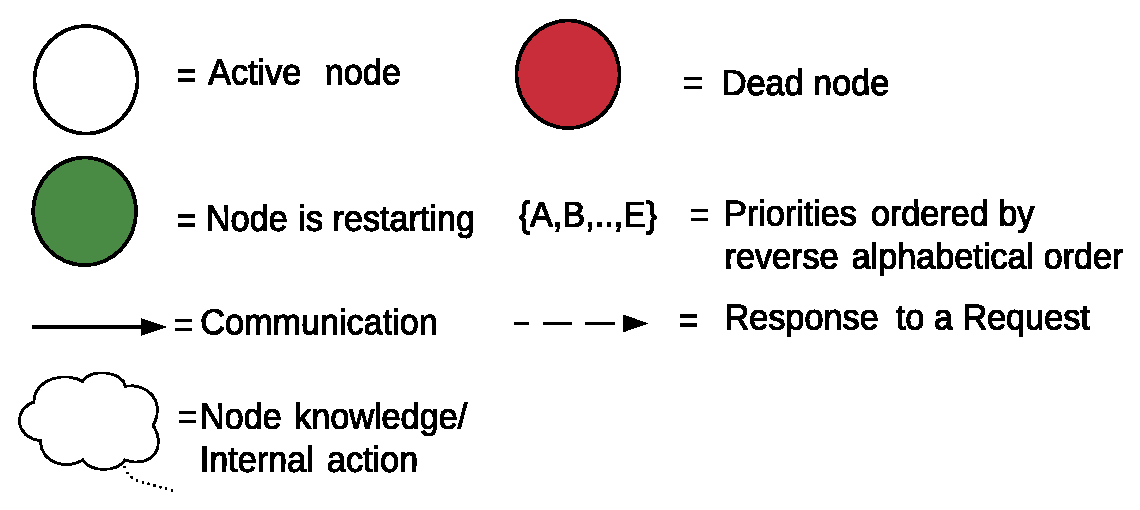
\includegraphics[width=.6\columnwidth]{images/solution/election_legend.eps}
%   \caption{Legend of \nameref{fig:election-protocol-ex}}
%   \label{fig:election-protocol-legend}
% \end{figure}

% \begin{figure}[H]
%   \centering
%   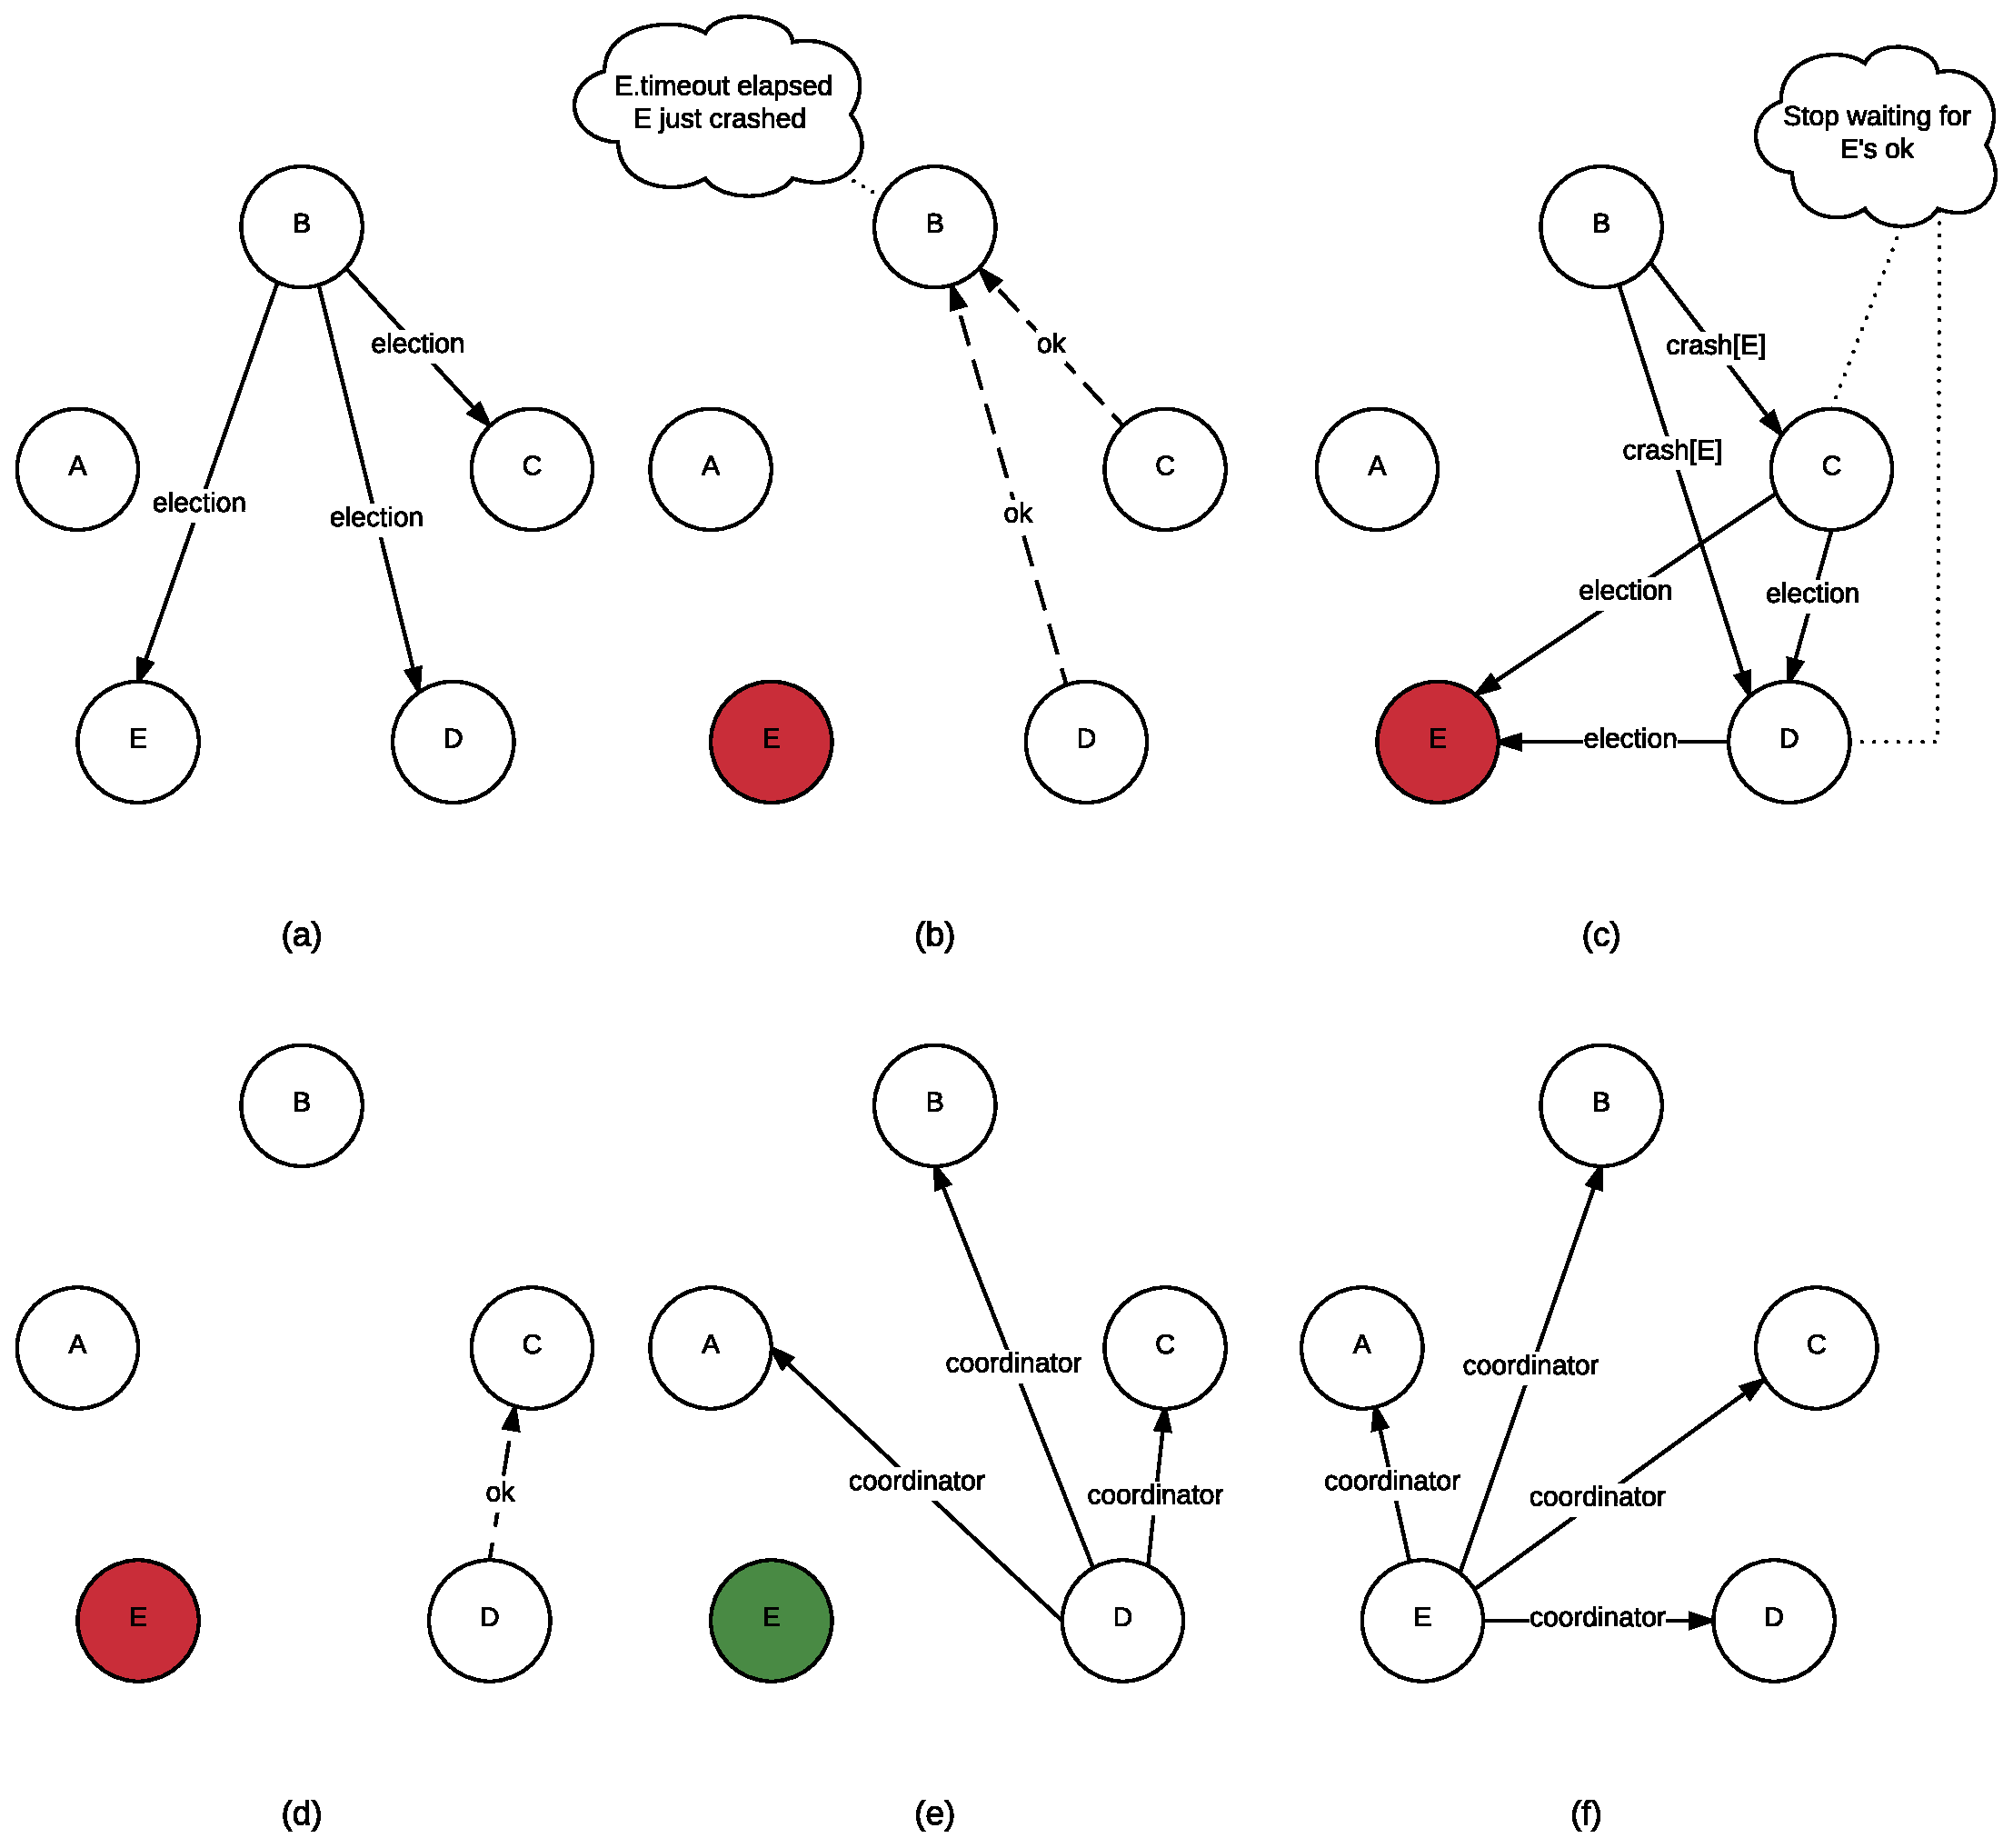
\includegraphics[width=\columnwidth]{images/solution/election.eps}
%   \caption{Election protocol - Example}
%   \label{fig:election-protocol-ex}
% \end{figure}

\subsubsubsection{System Boostrap}\label{sec:sys-boot-mw}
As pointed out in Problem Analysis (Section \ref{sec:pa-distribution}),
the system has
to start neatly. Hence, we need to design a protocol in order to accomplish
this goal.

The protocol is represented in Figure \ref{fig:sys-bootstrap-protocol}, where:

\begin{itemize}
  \item A circle is a logical node which is composed of two layers:
    \begin{itemize}
      \item \textbf{MW}:  middleware layer
      \item \textbf{APP}: application layer
  \end{itemize}
  \item \textbf{Named arrow}: it represents a message that is sent from a
logical node through another one with the name as its payload;
  \item \textbf{Number}: it represents the progress of the logical system clock
during the bootstrap process.
\end{itemize}

% TODO: Name leftmost node as 'l'
\begin{figure}[H]
  \centering
  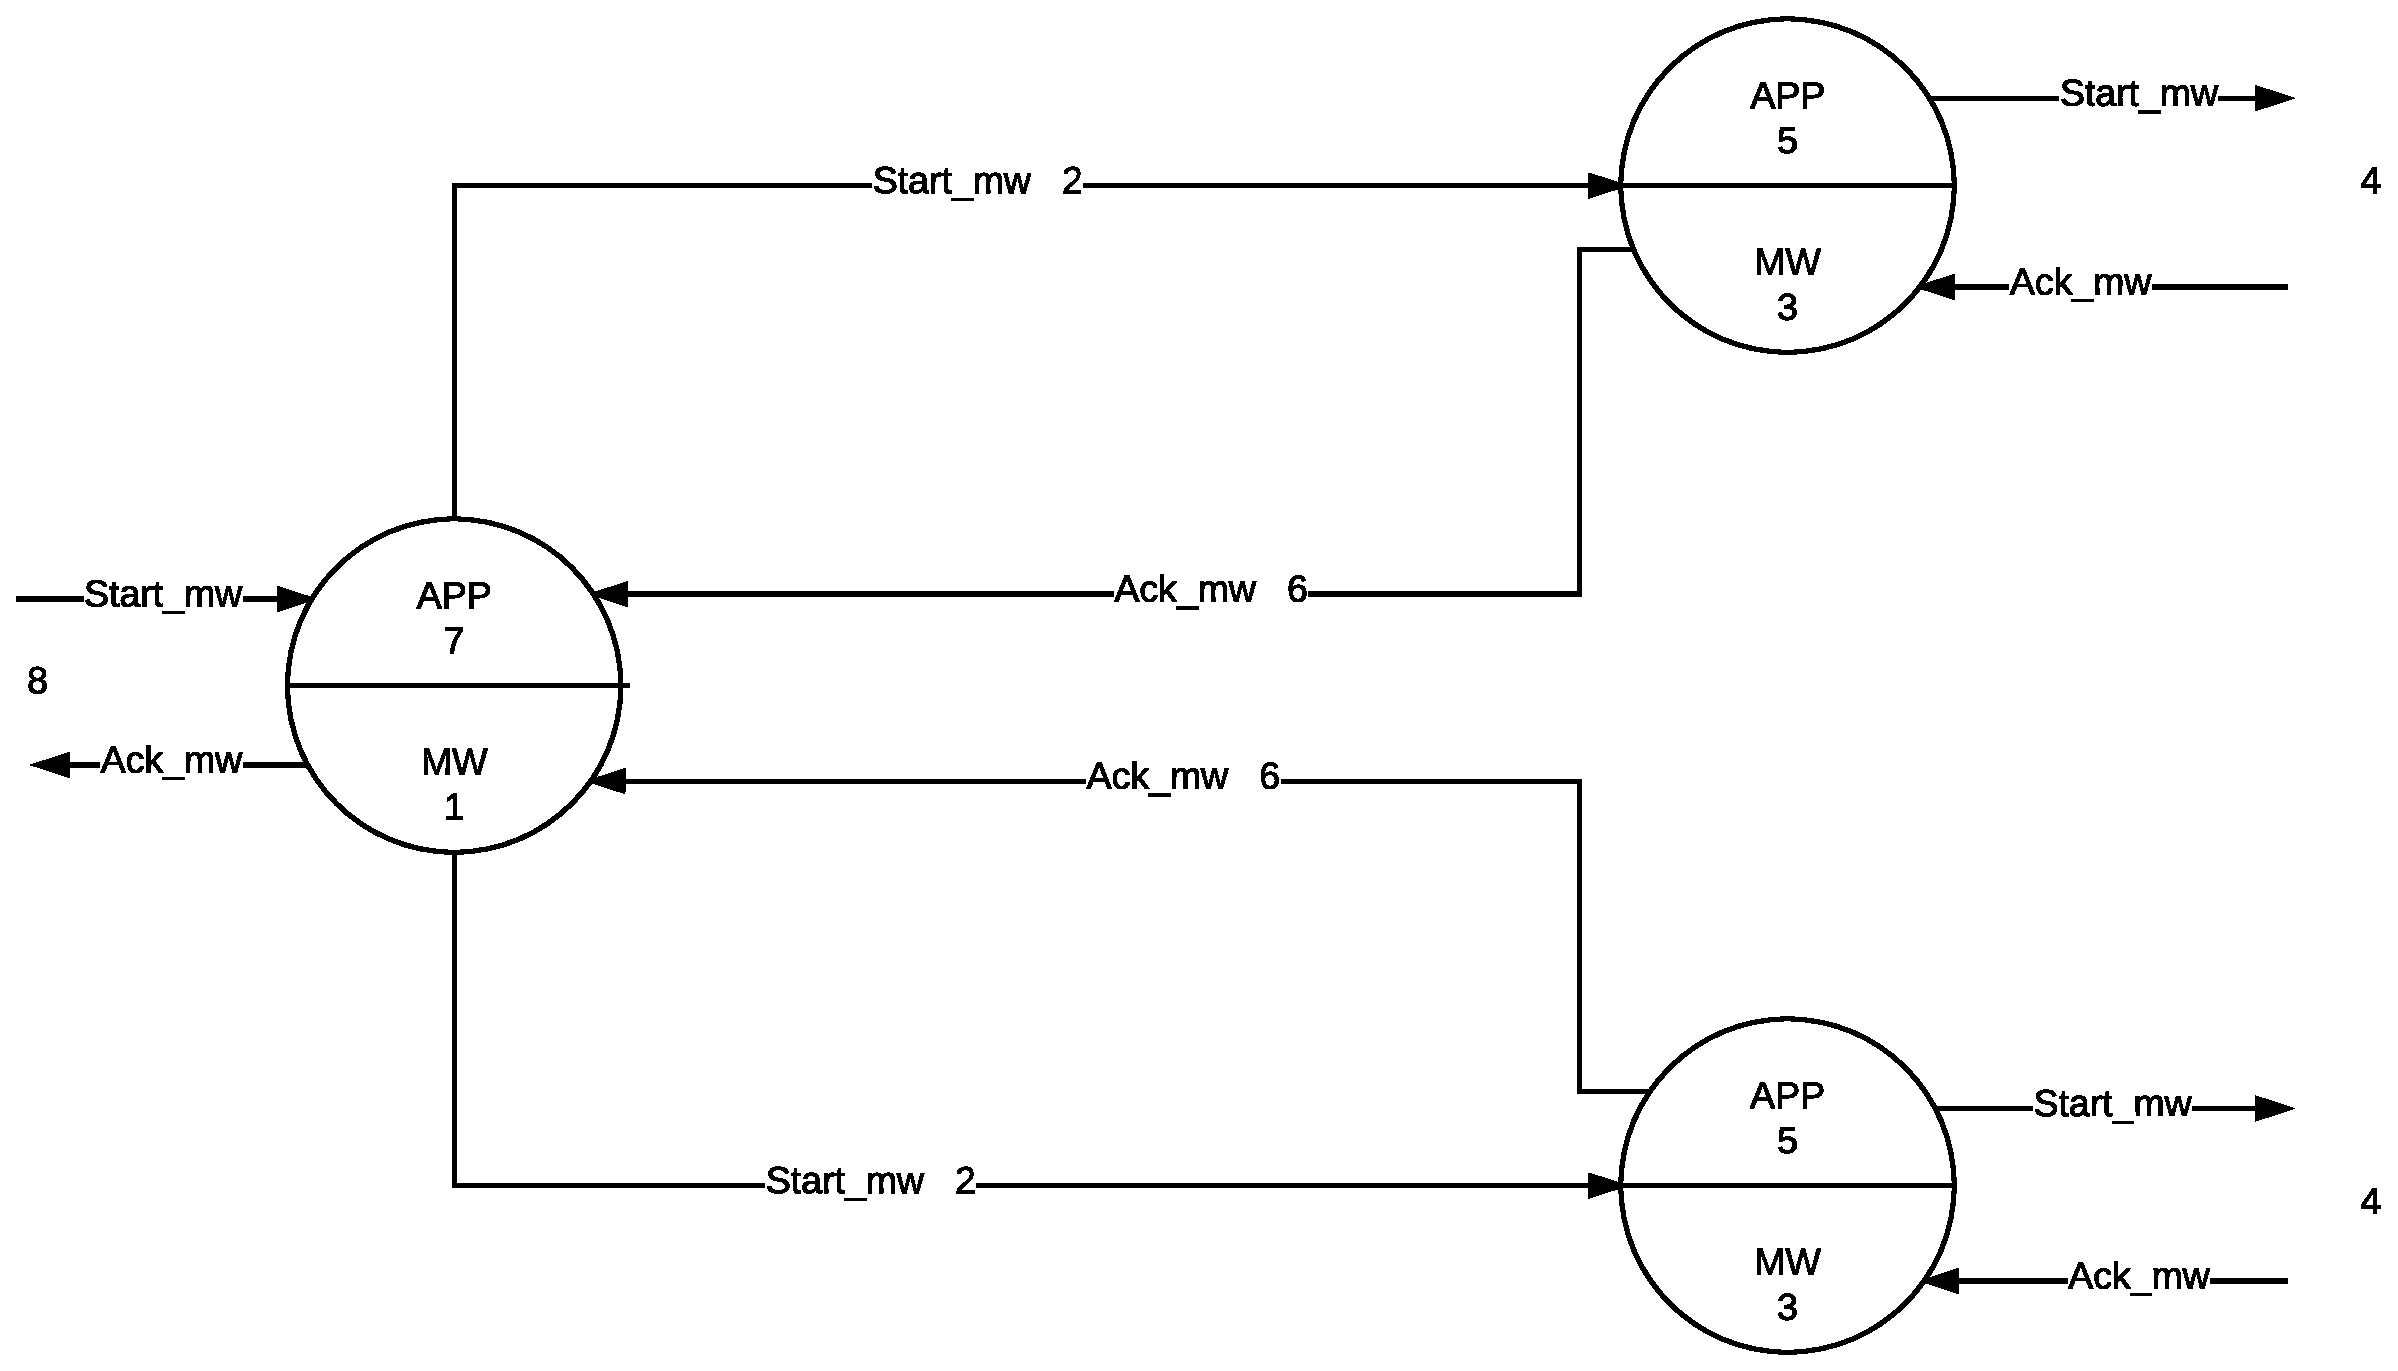
\includegraphics[width=\columnwidth]{images/solution/bootstrap.eps}
  \caption{System bootstrap protocol}
  \label{fig:sys-bootstrap-protocol}
\end{figure}

Assuming that a \texttt{Start\_mw} message arrives to a non-booted node (say
$l$) at time 0, the protocol is defined as follows:

\begin{enumerate}
\item The leftmost node $l$ in figure \ref{fig:sys-bootstrap-protocol}
  starts its own middleware services;
\item $l$ sends a \texttt{Start\_mw} message to the set $S$ of all its
  %TODO:         Is it really clear?
  %             /
  neighbors. Clearly, if it was the first node in the system to receive
  \texttt{Start\_mw}, then it will be also the last node to complete the
  boot process;
  % REPLY: Yes, it is clear (Stefano)
\item $l$ waits for each node in $S$ to complete the boot. $l$ waits for all
  nodes in $S$ to send an \texttt{Ack\_mw} message as a reply;
\item The middleware MW of $l$ grants the application APP to start;
\item $l$ then replies with an \texttt{Ack\_mw} message.
\end{enumerate}

As it can be seen in the figure, this behaviour is replicated recursively
by all nodes of the system. If a node has already received a boot request,
then it only sends \texttt{Ack\_mw} back.


\subsubsubsection{System Termination}\label{sec:comm-mw-termination}
The system has to shutdown neatly. Therefore we designed a protocol to
stop the entire system. This one can be seen as a
symmetric version of the System Bootstrap (\ref{sec:sys-boot-mw}).
% TODO: please check the sentence here above

The protocol is represented in figure \ref{fig:sys-termination-protocol}, where
the conventions are the same as the ones used in figure
\ref{fig:sys-bootstrap-protocol}.

% TODO: Name leftmost node as 'l'
\begin{figure}[H]
  \centering
  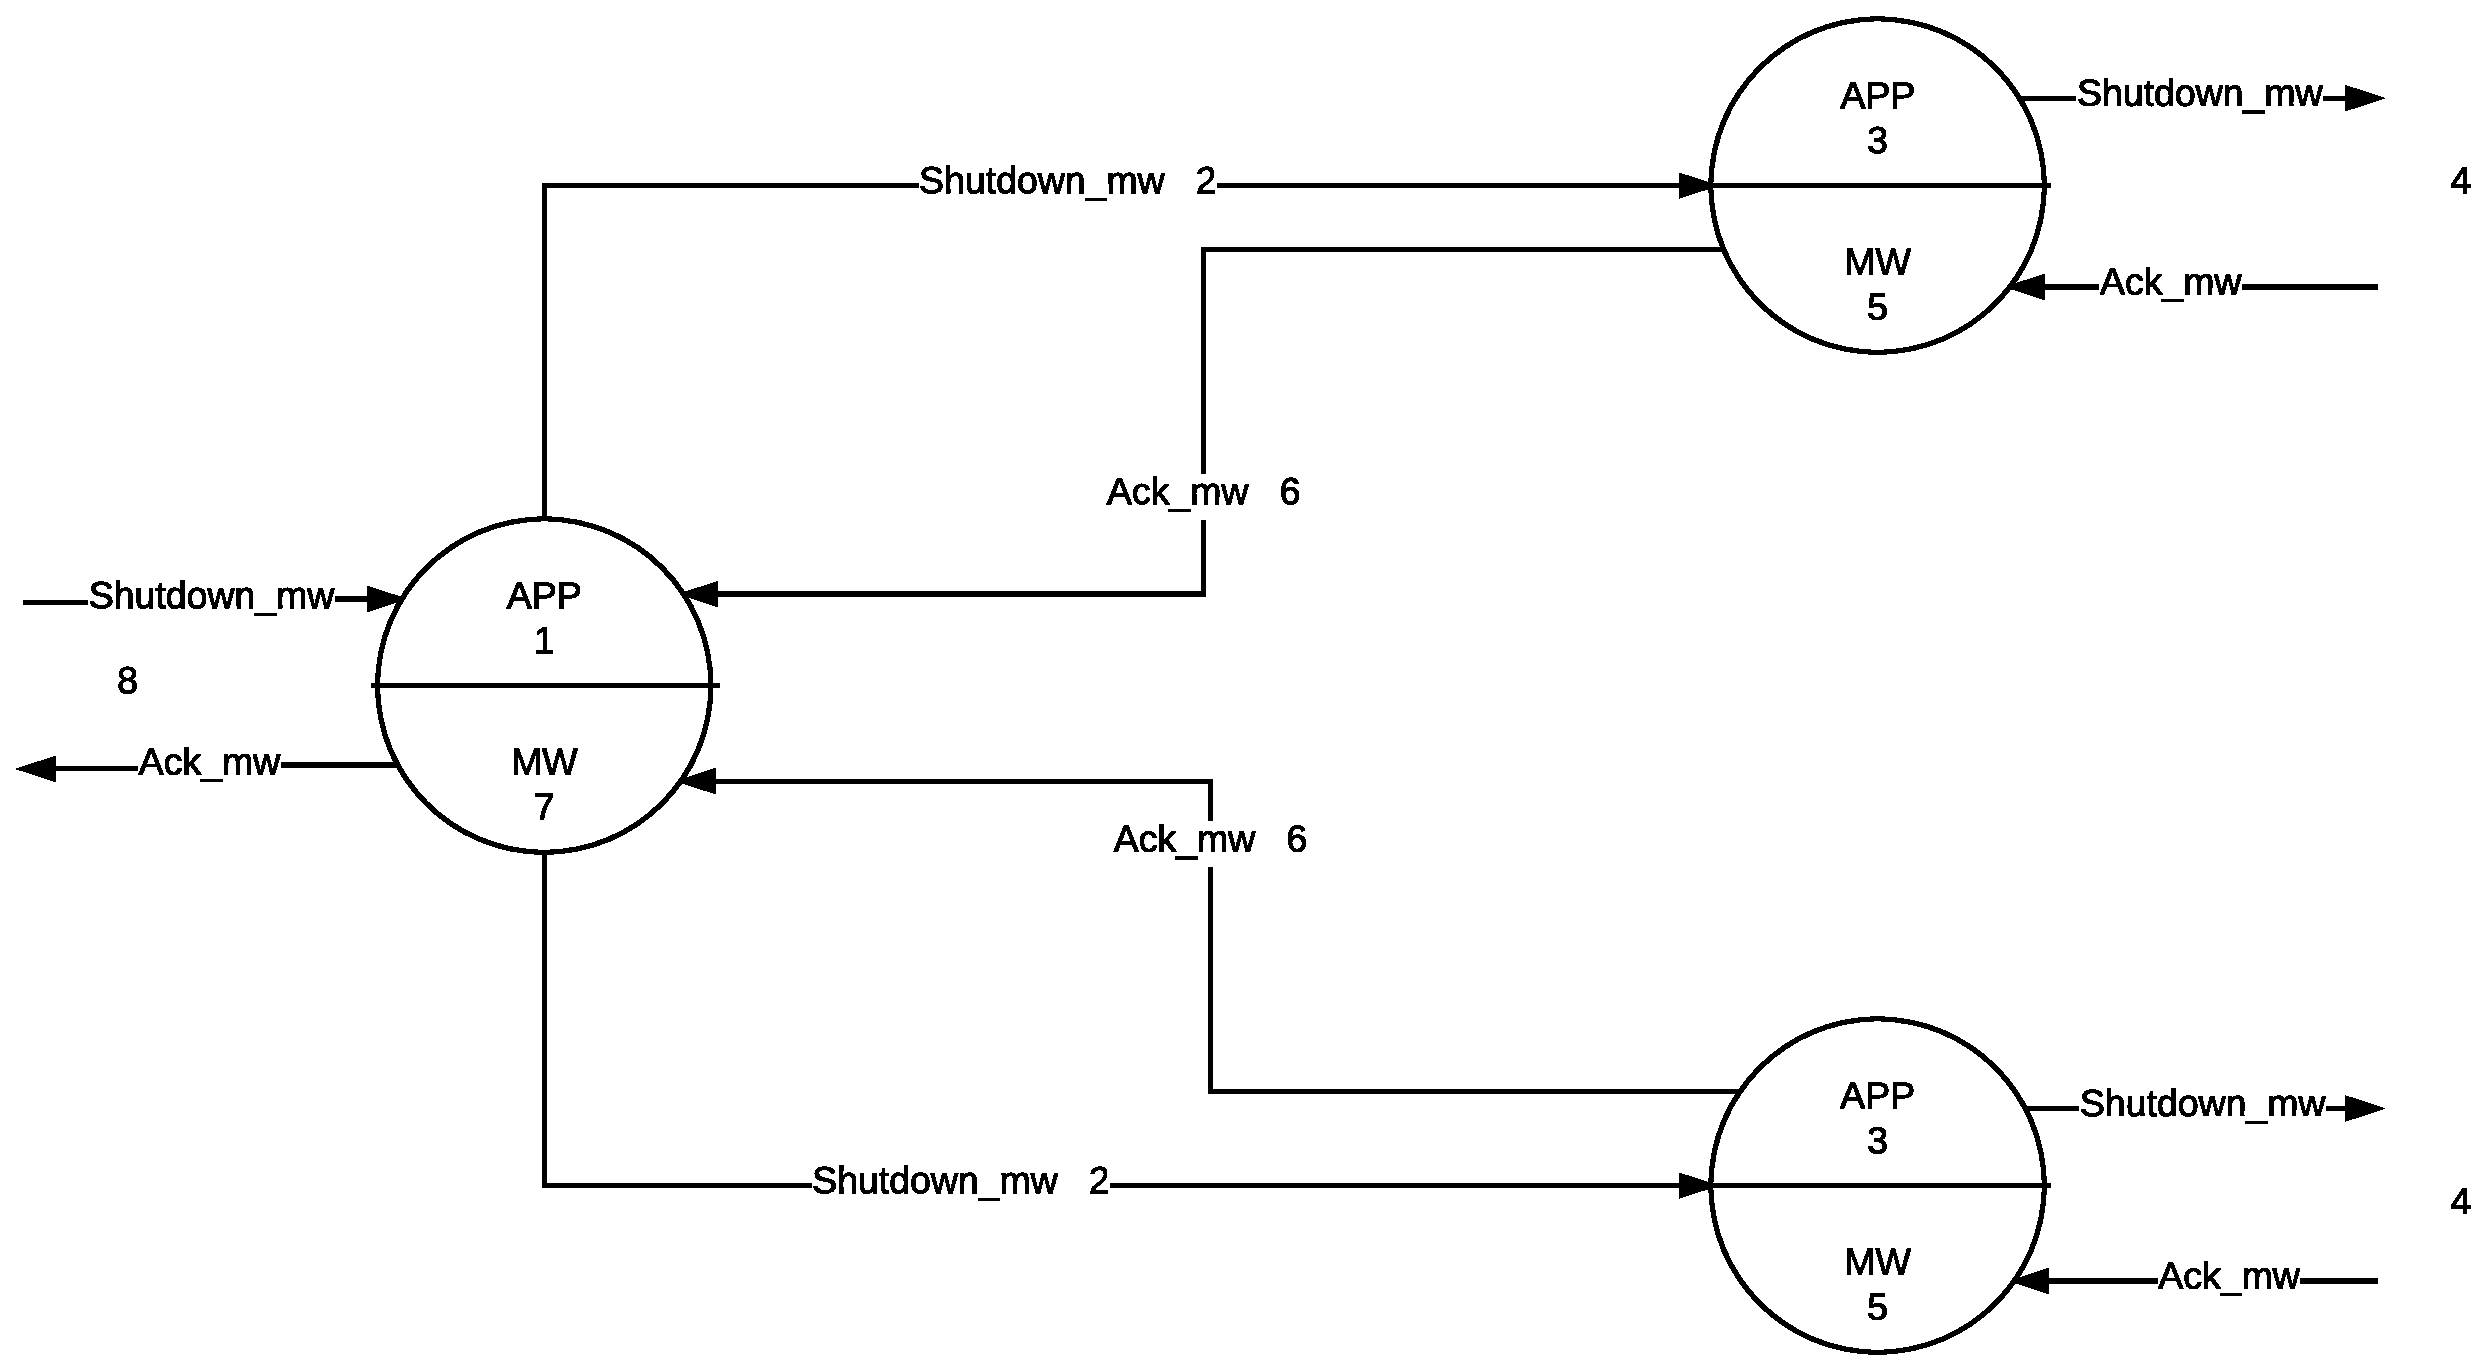
\includegraphics[width=\columnwidth]{images/solution/termination.eps}
  \caption{System termination protocol}
  \label{fig:sys-termination-protocol}
\end{figure}

Assuming that a \texttt{Shutdown\_mw} message arrives to a running node
$l$ (let it be the leftmost one in the picture) at time instant $0$, the
protocol is defined as follows:

\begin{enumerate}
\item The middleware MW of $l$ asks to terminate the application APP;
\item $l$ sends a \texttt{Shutdown\_mw} message to the set
  $S$ of all the nodes it knows;
\item $l$ waits for each node in $S$ to terminate, i.e. $l$ waits for all
  nodes in $S$ to send an \texttt{Ack\_mw} message back;
\item $l$ waits for its own application layer APP to stop;
\item $l$ stops its own middleware services;
\item $l$ then sends an \texttt{Ack\_mw} message back.
\end{enumerate}

As it can be seen in the related figure, this behaviour is replicated
recursively by all nodes of the system. If a node has already received a
termination request, then it only sends \texttt{Ack\_mw} back.
